
%(BEGIN_QUESTION)
% Copyright 2006, Tony R. Kuphaldt, released under the Creative Commons Attribution License (v 1.0)
% This means you may do almost anything with this work of mine, so long as you give me proper credit

Bruk Bernoulli's formel for å regne ut trykket $P_2$. Massetettheten til fluidet er $\rho = 800kg/m$
$$\includegraphics[width=15.5cm]{i00451x01.eps}$$

Bernoulli's formel:

\vskip 10pt

$$z_1 \rho g + {v_1^2 \rho \over 2} + P_1 = z_2 \rho g + {v_2^2 \rho \over 2} + P_2$$

\vskip 10pt

\noindent
Where,

$z$ = Height of fluid, in meter (m)

$\rho$ = Mass density of fluid, in kg per kubikkmeter (kg/m$^3$)

$g$ = Acceleration of gravity (9.81 m/s$^{2}$)

$v$ = Hastigheten til fluidet i meter per sekund (m/s)

$P$ = Trykket av fluidet i Pascal (Pa=N/m²) 

\vskip 10pt

Til slutt regn ut differansetrykket i dette venturi måleelementet. ($\Delta P$)
\vskip 10pt

\vskip 20pt \vbox{\hrule \hbox{\strut \vrule{} {\bf Suggestions for Socratic discussion} \vrule} \hrule}

\begin{itemize}
\item{} The textbook outlines a general strategy for generating a problem-solving plan when tackling problems with complex mathematical formulae.  Specifically, this strategy involved writing out the formulae and linking variables between formulae with arrow symbols.  Explain how this strategy works, and show how it may be applied to the solution of this problem.
\item{} A very helpful strategy for tackling Bernoulli's equation problems is to create a table in which to place each of the ``head'' terms of that equation.  Explain why this is helpful to manage this specific type of problem.
\item{} Venturi tubes are often used to create {\it vacuums}, by passing some fluid through the venturi at high speed and then providing a vacuum tap at the throat.  Automobile engine carburetors and atomizing spray guns are two prominent examples of this.  In industry, another example is the so-called {\it steam eductor}, using a jet of high-velocity steam through a venturi to create continuous suction (vacuum).  Are there any advantages to using eductors to create vacuums as opposed to using mechanical vacuum pumps?  Are there any disadvantages to the use of eductors for creating vacuums?
\end{itemize}

\underbar{file i00451}
%(END_QUESTION)





%(BEGIN_ANSWER)

$P_2$ = 0.018 MPa 

\vskip 10pt

Note: even slight amounts of rounding error may add up to skew the $P_2$ pressure calculation so that it ends up being as high as 1 PSI instead of half of a PSI.  In order to avoid incurring rounding errors, you must store all intermediate calculated results in your calculator's memory locations rather than write them on paper and re-enter them.  This is a good practice in general, not only because it avoids unnecessary rounding being introduced into your calculations, but also because it completely avoids simple keystroke errors!

%(END_ANSWER)





%(BEGIN_NOTES)

$$V_1=\frac{Q}{A_1}=\frac{0.4m^3/s}{\pi \frac{(0.3m)^2}{4}}=5.66m/s$$
$$V_2=\frac{Q}{A_2}=\frac{0.4m^3/s}{\pi \frac{(0.1175m)^2}{4}}=36.89m/s$$

$$\cancel{z_1 \rho g} + {v_1^2 \rho \over 2} + P_1 = \cancel{z_2 \rho g} + {v_2^2 \rho \over 2} + P_2$$
$$P_2={v_1^2 \rho \over 2} + P_1 - {v_2^2 \rho \over 2}=\frac{(5.66m/s)^2\cdot 800kg/m³}{2}+0.55MPa-\frac{(36.89m/s)^2\cdot 800kg/m^3}{2}=-531504Pa$$


%INDEX% Physics, dynamic fluids: Bernoulli's equation

%(END_NOTES)


